% Insert early so the single-column float can occupy the first page's
% right-column top, alongside the abstract, using standard ACM float placement.
\noindent\textbf{Relevance Statement.}
This work is relevant to the Web Infrastructure and Agentic Systems track. Web agents use reusable task instructions, or skills, to guide actions across requests and services. Reusing the internal states formed from these instructions could help carry task capabilities across executions. We examine when such transfer weakens despite the original execution's continued dependence on the skill, and how the key/value caches used by attention can partly restore transfer. These findings inform the design and evaluation of reusable skill representations and context management for Web agents.


\begin{figure}[t]
\centering
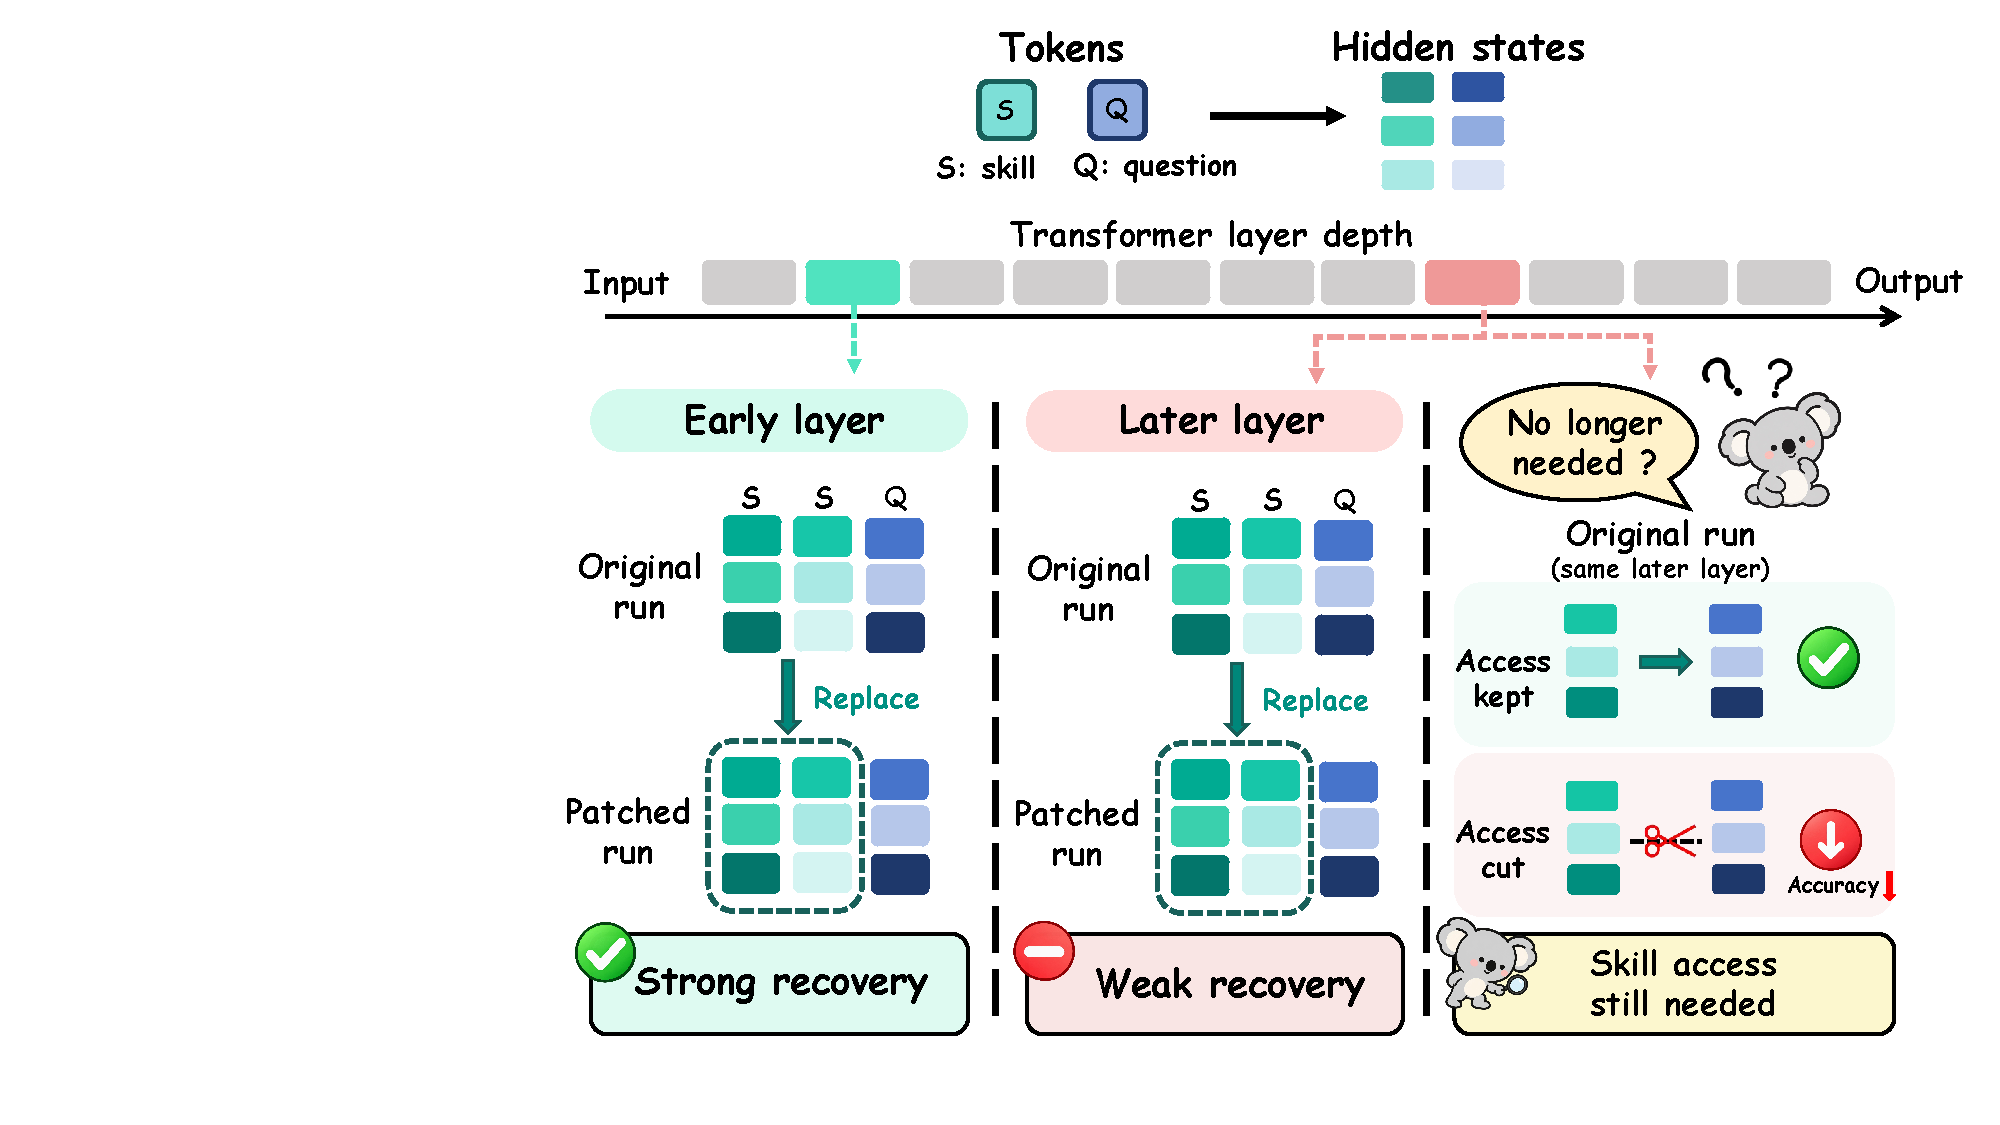
\includegraphics[width=\columnwidth]{fig-teaser.pdf}
\caption{Weak transfer and continued skill use at the same later depth.
Copying skill-position states from a correct-skill run into an unrelated-skill
run gives strong early recovery (left) and weak late recovery (middle).
At that same later depth, the original run still needs skill access:
retaining access preserves performance, while cutting it reduces accuracy
(right). S and Q label skill and question tokens.
Figure~\ref{fig:transferreading} gives the measured depth profiles.}
\Description{A schematic follows transformer depth from input to output.
At an early layer, replacing skill-position hidden states yields strong
recovery. At a later layer the same type of replacement yields weak recovery.
In the original correct-skill run at that later layer, retaining skill access
preserves performance while cutting access reduces accuracy. Green blocks
represent skill tokens and blue blocks question tokens.}
\label{fig:teaser}
\end{figure}

\section{Introduction}
\label{sec:intro}

Language models can perform new tasks by following instructions in their
context. A skill makes such instructions reusable: a calculator skill,
for example, specifies a formula, input conventions and the steps for
applying them to a new question. A model divides text into tokens and
represents each position with an internal vector, or hidden state.
If the hidden states formed from these
instructions also support reuse, one execution could supply task-relevant
information to another without changing the model's weights.

Agent Skills organize instructions, scripts and resources around a
\texttt{SKILL.md} entry point \citep{zhang2025agentskills}.
Web agents use reusable skills and workflows to guide later actions
\citep{wang2024awm,wang2026webxskill}. This motivates studying whether the
internal states formed from such instructions can also be reused. We
study this question through controlled question answering after a skill
has been selected, isolating the use and transfer of its instructions.

The difficulty is interpreting a failed transfer. If copying a skill's
hidden states no longer restores performance, has the model stopped
needing those instructions, or has the copy failed to supply what the
receiving execution needs? Task vectors summarize task demonstrations,
while function vectors combine selected internal attention outputs.
Both show that internal states can transmit task behaviour across contexts
\citep{hendel2023taskvectors,todd2024functionvectors}. Yet restoring an
execution and disrupting a successful one measure different effects
\citep{heimersheim2024patching}. This motivates our central question:
\emph{can skill-state transfer weaken while the original execution still
relies on access to the skill?}

We answer this question with two tests across model depth. The first
copies hidden states at the skill's token positions from a correct-skill
execution into an execution using length-matched text from an unrelated skill. The
second blocks attention to the skill in the original correct-skill
execution, from a chosen layer onward. Content, position and cross-question
controls first establish that early copying transfers skill-relevant
information. We then find a consistent separation in eight evaluated
combinations of four models and two benchmarks: transfer weakens at later
layers while the original execution remains strongly dependent on skill
attention (Figure~\ref{fig:teaser}).

We next test whether adding information omitted by hidden-state copying
can improve late transfer. Attention stores information from previously
processed tokens in a key/value (KV) cache. At layer $16$, copying these
caches together with hidden states improves accuracy over state transfer
alone in all eight settings, by $6.8$ to $43.4$ percentage points.
Blocking subsequent skill reading reduces the recovered accuracy in each
setting. For Qwen3-8B/MedCalc, joint replacement raises accuracy from
$3.5\%$ to $42.1\%$, and the reading cut reduces it to $7.0\%$.
The shared direction across models and tasks establishes cache-assisted
partial restoration alongside continued use of the skill.

Additional complete-source controls show that copying every layer of skill-position KV is still insufficient to reproduce the donor. Copying the complete prefix KV reproduces donor outputs, while the early-versus-late joint-repair pattern varies across models and tasks.

The paper follows three steps: validate early transfer
(\S\ref{sec:battery}), establish its separation from continued skill use
(\S\ref{sec:depth}), and test the extent of cache-assisted restoration
(\S\ref{sec:mechanism}). Together, the tests distinguish the ability to
use contextual instructions from the ability to reuse their internal
states, and identify cached information as a component that improves reuse.
